\subsection{A Baseline System}

For this paper, I solve the system in \autocites{othmer2009intersection}{jeong2017numerical}. By replacing the reaction function, the method can be extended to any sufficiently smooth reaction diffusion system. This includes Turing's initial version \parencites{turing1990chemical}{de2020leopard} and other activator-inhibitor equations \parencites{landge2020pattern}{meinhardt2000pattern} which it has been tested against. The system I solve is given by
\begin{align*}
    \frac{\partial u}{\partial t} = \gamma_u \nabla^2 u + k_1 \left(v - \frac{uv}{1 + v^2}\right) \\
    \frac{\partial v}{\partial t} = \gamma_v \nabla^2 v + k_2 - v - \frac{4 u v}{1 + v^2}.
\end{align*}

Like \autocite{jeong2017numerical}, I fix $D_u = 1$ and $k_2 = 11$ in all simulations. I vary $D_v$ and $k_1$ across simulations to create different Turning patterns, but we always have $D_v< D_u$. The time step is set to $\Delta t = 0.01$, and all systems are iterated until $t = 1,000$, at which point they all have reached a steady state. I triangulate so that there are 250 points per square unit of the domain I solve the PDE on. The plotted solutions will be of $u$, although $v$ makes a similar pattern.


\subsection{Solutions}

\begin{figure}[t!]
    \centering
    \caption{Solutions to the reaction diffusion system}

    \begin{subfigure}{\textwidth}
        \centering
        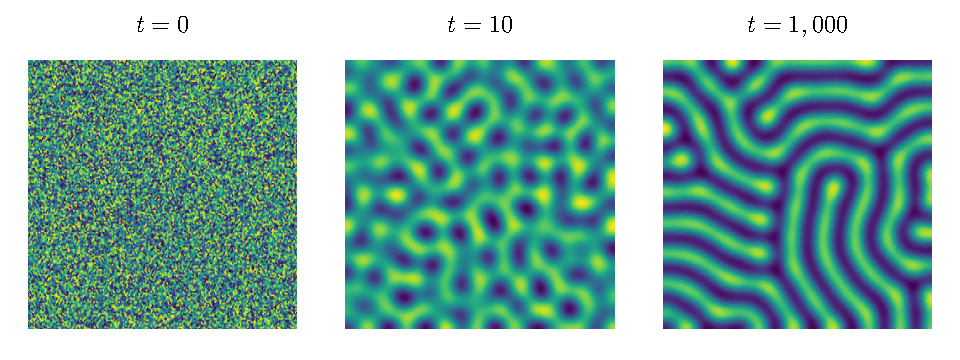
\includegraphics{figures/square_ts.pdf}
        \caption{$10 \times 10$ square domain}
    \end{subfigure}

    \begin{subfigure}{\textwidth}
        \centering
        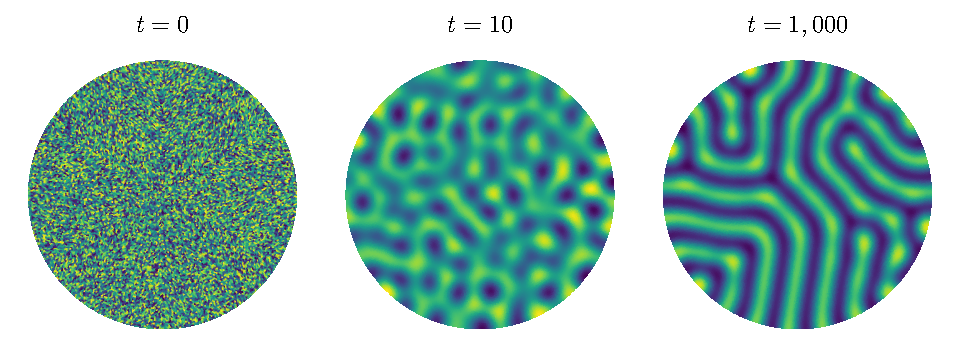
\includegraphics{figures/circle_ts.pdf}
        \caption{Radius 5 circular domain}
    \end{subfigure}
    \label{fig:sol-ts}
\end{figure}

Figure \ref{fig:sol-ts} plots the solution to the reaction diffusion system at different time steps on a square and circular domain. The left panel plots the initial condition, the middle panel plots an intermediate step during the reaction, and the right panel plots the system at steady state. I set the initial condition to random noise. At $t = 10$, the reaction starts to progress, and we see patterns and `hotspots' emerge. The patterns that exist, however, lack clear definition. In the steady state, we see well-defined lines that form clear Turing patterns.

At each time step, the system makes similar shapes on the circular and square domains. The intermediate step patterns both have similarly sized hotspots, and the Turing patterns that develop have a similar structure being made of curved-lines with similar width. I explore this further in Section \ref{sec:doms} with more complicated domains and arrive at the same result.


\subsection{Parameters}

\begin{figure}[t!]
    \centering
    \caption{$10 \times 10$ square steady states for different $\gamma_v$ and $k_1$}
    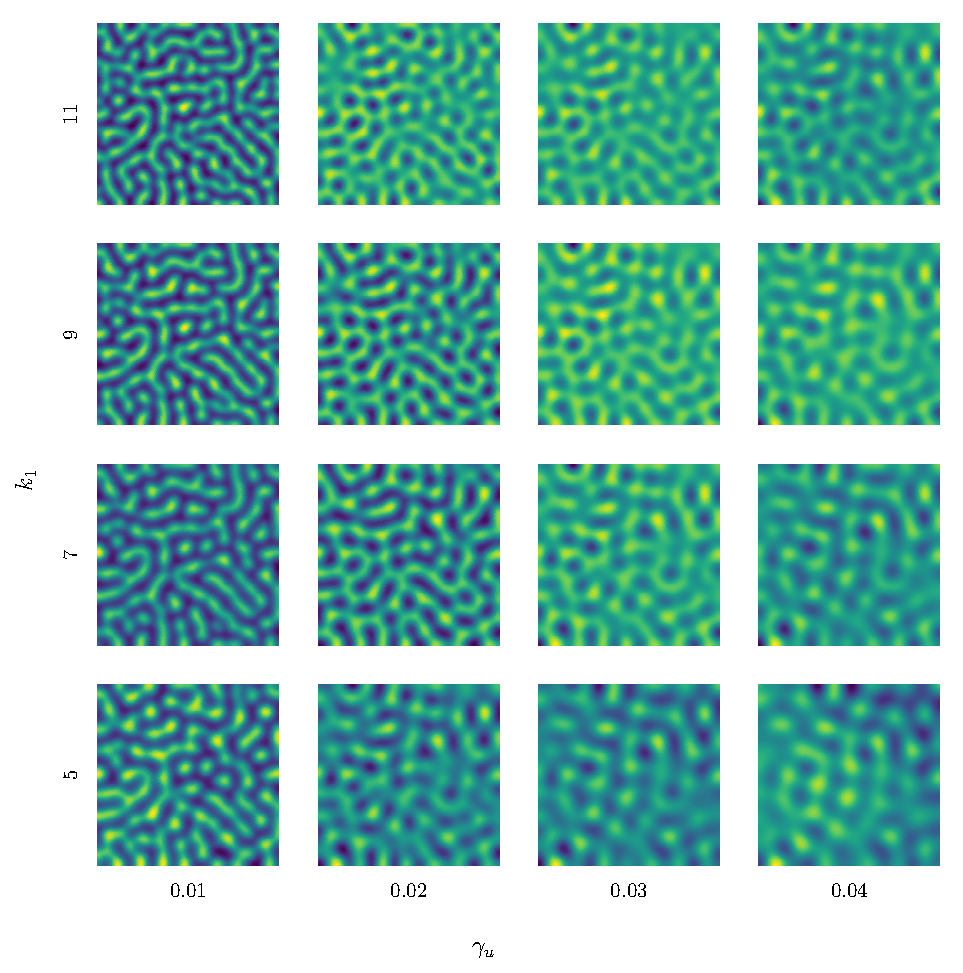
\includegraphics{figures/square_params.pdf}
    \label{fig:sq-pars}
\end{figure}

\begin{figure}[t!]
    \centering
    \caption{Radius 5 circle steady states for different $\gamma_v$ and $k_1$}
    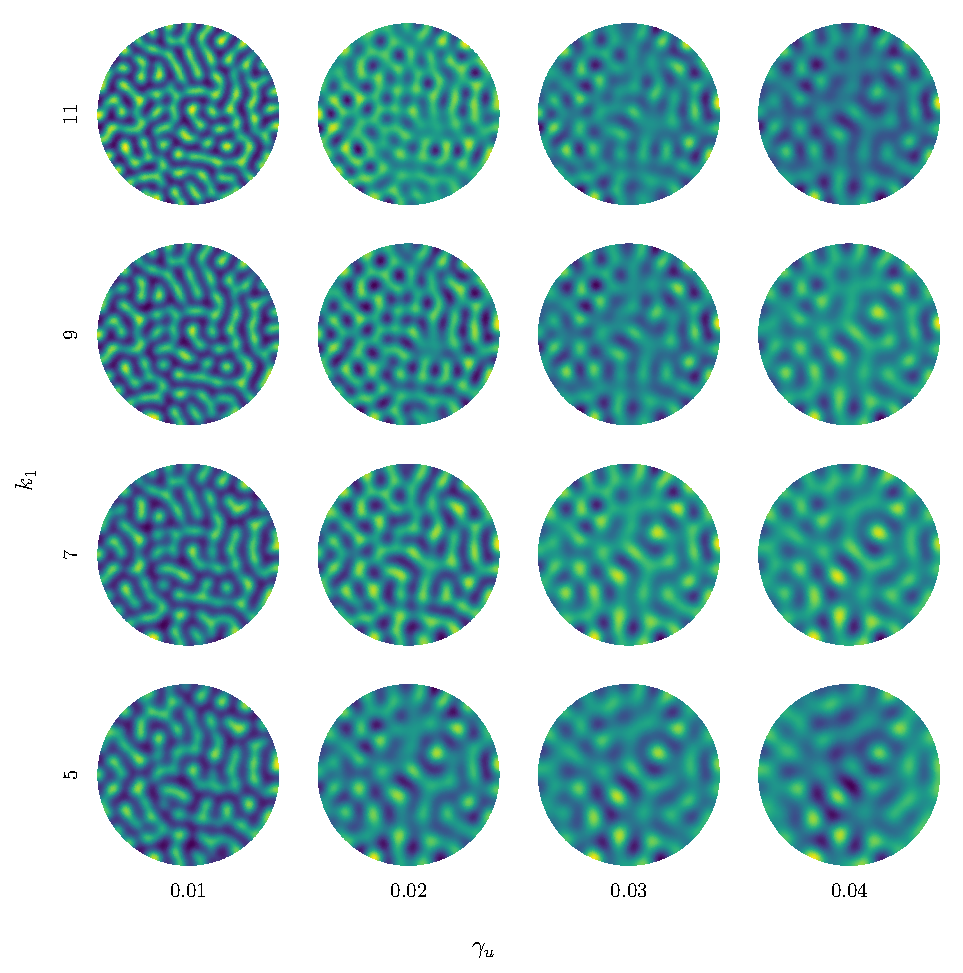
\includegraphics{figures/circle_params.pdf}
    \label{fig:cir-pars}
\end{figure}










